\documentclass[11pt]{article}
\usepackage[margin=1.05in,headheight=14pt]{geometry}
\usepackage[T1]{fontenc}
\usepackage{lmodern,microtype,amsmath,amssymb,amsthm,booktabs,tikz}
\usepackage{xcolor}
\definecolor{linknavy}{RGB}{25,55,125}
\usepackage[colorlinks=true,linkcolor=linknavy,citecolor=linknavy,urlcolor=linknavy]{hyperref}
\usepackage{orcidlink,fancyhdr}
\newtheorem{theorem}{Theorem}
\newtheorem{lemma}[theorem]{Lemma}
\newtheorem{corollary}[theorem]{Corollary}
\theoremstyle{remark}
\newtheorem{remark}[theorem]{Remark}
\newcommand{\e}{\mathrm{e}}
\pagestyle{fancy}
\fancyhf{}
\fancyhead[L]{\small CAOS Research Preprint}
\fancyhead[R]{\small Next matching level\textperiodcentered\ v0.01}
\fancyfoot[C]{\thepage}
\fancypagestyle{plain}{\fancyhf{}\fancyfoot[C]{\thepage}\renewcommand{\headrulewidth}{0pt}}
\title{The next matching level for triangle-free\\graphs with bounded degree}
\author{Felipe Santiba\~nez-Leal\,\orcidlink{0000-0002-0150-3246}\\
\small CAOS Research program\\
\small\texttt{github.com/fsantibanezleal/CAOS\_RESEARCH}}
\date{2026-09-05\\[2pt]\normalsize Version 0.01}
\begin{document}
\maketitle
\begin{center}\small
\fbox{\parbox{0.92\textwidth}{\centering
\textbf{PREPRINT}\textperiodcentered\ not peer reviewed\textperiodcentered\ CAOS Research\\
Bougard--Joret research series, second paper\textperiodcentered\ v0.01\\
\href{https://doi.org/10.5281/zenodo.22343021}{Concept DOI: 10.5281/zenodo.22343021} (latest version)\\
CC BY 4.0\textperiodcentered\ \href{https://github.com/fsantibanezleal/CAOS_RESEARCH}{Public sources and exact verification record}
}}
\end{center}
\begin{abstract}
Let $T(d,m)$ be the maximum number of edges in a triangle-free graph with maximum degree at most $d$ and matching number at most $m$, with no restriction on its order. We prove
$T(d,d+1)=d^2+d+2$ for every integer $d\ge7$.
A shortest-odd-cycle deficit bound, followed by a five-type equality obstruction, first gives the same maximum on $2d+3$ vertices. The Tutte--Berge formula extends this bound to arbitrary order.
The attaining construction is due to Banak, Ekim and Ta\c{s}k\i n; the contribution is the uniform upper bound. This settles the next-matching slice of the Ahanjideh--Ekim--Y\i ld\i z conjecture and, in particular, resolves the published bounds $184\le T(13,14)\le185$ in favor of 184.
As a consequence, we obtain a one-edge bracket for the Bougard--Joret extremal function at $(n,\alpha,k)=(2d+3,2,d+2)$, giving an unbounded strict-interior discrepancy from the degree-sum prediction. The full AEY conjecture and the exact endpoint of that bracket remain unresolved. Exact finite certificates and independent implementation checks support, but do not replace, the proof.
\end{abstract}

\section{Problem and relation to prior work}

All graphs are finite, simple and undirected. Write $\e(F)$, $\Delta(F)$ and $\nu(F)$ for the number of edges, maximum degree and maximum matching size of $F$. Define
\[
T(d,m)=\max\{\e(F): F\text{ triangle-free},\ \Delta(F)\le d,\ \nu(F)\le m\}.
\]
Isolated vertices are allowed and have no effect on the maximum. We use $T$ to distinguish this function from the Bougard--Joret minimum-edge function in Section~\ref{sec:bj}.

Ahanjideh, Ekim and Y\i ld\i z (AEY) study this degree/matching problem and conjecture, in their intermediate range $d<i<Z(d)$, that $T(d,i)=di+i-d+1$~\cite[Conjecture 6.1]{AEY}. Here $Z(d)$ is their threshold for a triangle-free factor-critical graph with their extremal degree sequence. Our result concerns the complete next level $i=d+1$ for $d\ge7$.

Banak, Ekim and Ta\c{s}k\i n (BET) provide the attaining family in Proposition~4.1 and computationally resolve a substantial finite range~\cite{BET}. Their Table~3 already determines $T(d,d+1)$ for $d=7,\ldots,12$. At $(d,m)=(13,14)$ it reports lower bound 184 and upper bound 185. Those finite results and the construction are prior work. The new conclusion here is the uniform upper bound, including
\[
T(13,14)=184.
\]
The source comparison used AEY's final published text and BET's complete author manuscript; BET's final publisher PDF was not obtained. Additional searches located no explicit prior uniform solution of this slice, without establishing exhaustive bibliographic priority.

Regular triangle-free extremal results, including Caro--Tuza~\cite[Theorem 2(iii)]{CT} and the later regular Tur\'an literature~\cite{CDK}, already imply strong regular-degree obstructions. They are not asserted as new here. Our fixed-order theorem permits nonregular graphs with maximum degree at most $d$; its attaining graph has one vertex of degree four and all other vertices of degree $d$.

\begin{theorem}[Next matching level, D]\label{thm:main}
For every integer $d\ge7$,
\[
T(d,d+1)=d^2+d+2.
\]
\end{theorem}

Our universal deductions are labeled [D] and exact finite checks [MV]. The proof and certificates form EXP-003 of the public record~\cite{Record}. This paper is separate from the earlier first-shell Bougard--Joret preprint~\cite{Shell}, which remains unchanged.

\section{The fixed-order upper bound}

\begin{lemma}[Shortest odd cycle]\label{lem:cycle}
Let $F$ be triangle-free on $n$ vertices and let $C$ be a shortest odd cycle, of length $\ell$. Then $\ell\ge5$, $C$ is chordless, every vertex outside $C$ has at most two neighbors on $C$, and
\[
\sum_{x\in V(C)}\deg_F(x)\le2n.
\]
\end{lemma}
\begin{proof}
Triangle-freeness gives $\ell\ge5$. A chord would split $C$ into two cycles of opposite parity, producing a shorter odd cycle.
If an outside vertex has at least three neighbors on $C$, list all of them in cyclic order. The intervening arc lengths sum to the odd number $\ell$, so at least one arc is odd. Every arc has length at least two, by triangle-freeness. The other arcs have total length at least four, so the odd arc has length at most $\ell-4$. Adding the two edges to the outside vertex produces an odd cycle of length at most $\ell-2$, a contradiction.
The cycle contributes $2\ell$ to its degree sum and the $n-\ell$ outside vertices contribute at most $2(n-\ell)$, proving the bound.
\end{proof}

If $\Delta(F)\le d$, its total degree deficit is
\[
D(F)=\sum_{x\in V(F)}(d-\deg_F(x))=nd-2\e(F).
\]
Every summand is nonnegative. For nonbipartite $F$, Lemma~\ref{lem:cycle} yields
\begin{equation}\label{eq:deficit}
D(F)\ge\sum_{x\in V(C)}(d-\deg_F(x))
\ge\ell d-2n\ge5d-2n.
\end{equation}

\begin{theorem}[Fixed order, D]\label{thm:order}
For every integer $d\ge7$, the maximum number of edges in a triangle-free graph on $2d+3$ vertices with maximum degree at most $d$ is $d^2+d+2$.
\end{theorem}
\begin{proof}[Proof of the upper bound]
Let $n=2d+3$. If $F$ is bipartite, one part has at most $d+1$ vertices, so summing degrees on that part gives $\e(F)\le d(d+1)$.
Otherwise~\eqref{eq:deficit} gives $D(F)\ge d-6$ and therefore
\begin{equation}\label{eq:oneedge}
\e(F)\le d^2+d+3.
\end{equation}
Suppose equality holds. Then every inequality in~\eqref{eq:deficit} is an equality. Thus a shortest odd cycle has length five, every outside vertex has degree exactly $d$, and every outside vertex has exactly two neighbors on the cycle.

Number the cycle $c_0,\ldots,c_4$, with indices modulo five. Its two neighbors at an outside vertex must form a nonadjacent pair, uniquely $\{c_{i-1},c_{i+1}\}$ for some $i$. Let $V_i$ contain $c_i$ and all outside vertices with this pair, and put $n_i=|V_i|$. Then
\begin{equation}\label{eq:types}
n_i\ge1,\qquad \sum_i n_i=2d+3.
\end{equation}
Each $V_i$ is independent, and there are no edges between $V_i$ and $V_{i+2}$: such vertices share a cycle neighbor. Every possible edge therefore joins consecutive types. We do not assume completeness between types.

By definition, $c_i$ is adjacent to every member of $V_{i-1}\cup V_{i+1}$ and no others. Hence
\begin{equation}\label{eq:b}
b_i:=n_{i-1}+n_{i+1}=\deg_F(c_i)\le d.
\end{equation}
If $n_i\ge2$, an outside vertex in $V_i$ has degree $d$ and all its neighbors lie in the two adjacent types. Thus
\begin{equation}\label{eq:large}
n_i\ge2\quad\Longrightarrow\quad b_i=d.
\end{equation}

These constraints are impossible for $d>6$. If every $n_i\ge2$, summing~\eqref{eq:large} gives $5d=2\sum_i n_i=4d+6$, so $d=6$. Otherwise rotate indices so that $n_0=1$.

If $n_1,n_4\ge2$, equation~\eqref{eq:large} gives $n_2=n_3=d-1$. The total in~\eqref{eq:types} forces $n_1+n_4=4$, so $n_1=n_4=2$. But then $b_2=n_1+n_3=d+1$, contradicting~\eqref{eq:b}.

We may therefore reflect indices and assume $n_0=n_1=1$. If $n_2,n_4\ge2$, equation~\eqref{eq:large} gives $n_3=d-1$. Now~\eqref{eq:types} forces $n_2+n_4=d+2$, contrary to $b_3\le d$.

Otherwise there are three consecutive singleton types; after relabeling, $n_0=n_1=n_2=1$. Then $n_3+n_4=2d$, while~\eqref{eq:b} at types 0 and 2 gives $n_4,n_3\le d-1$, another contradiction.

Equality in~\eqref{eq:oneedge} is impossible. Integrality improves the upper bound to $d^2+d+2$. No parity assumption was used. Attainment is proved in Section~\ref{sec:attain}.
\end{proof}

\begin{figure}[ht]
\centering
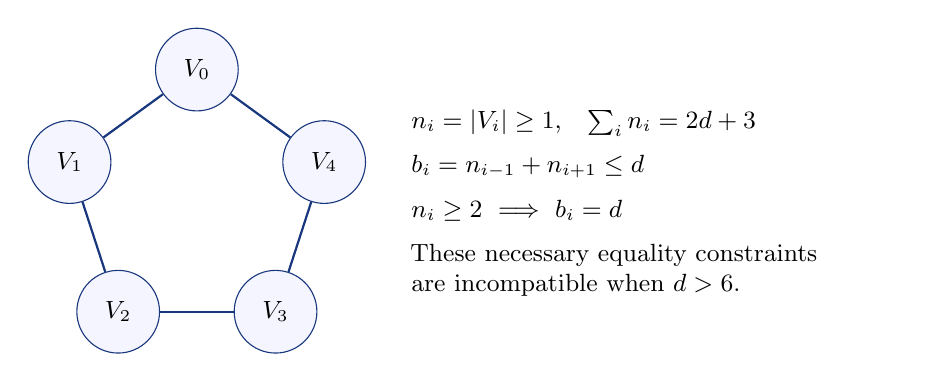
\begin{tikzpicture}[scale=1.0,every node/.style={font=\small}]
\foreach \i in {0,...,4}{
  \node[draw=linknavy,fill=blue!4,circle,minimum size=1.05cm] (v\i) at ({90+72*\i}:1.7) {$V_\i$};
}
\foreach \i/\j in {0/1,1/2,2/3,3/4,4/0}{\draw[thick,linknavy] (v\i)--(v\j);}
\node[align=left,anchor=west,text width=6.2cm] at (2.6,0) {
$n_i=|V_i|\ge1$,\quad $\sum_i n_i=2d+3$\\[5pt]
$b_i=n_{i-1}+n_{i+1}\le d$\\[5pt]
$n_i\ge2\ \Longrightarrow\ b_i=d$\\[5pt]
These necessary equality constraints\newline are incompatible when $d>6$.};
\end{tikzpicture}
\caption{The five-type obstruction. Lines show allowed adjacencies, not an assumption of complete bipartite adjacency.}
\label{fig:types}
\end{figure}

\section{The known attaining construction}\label{sec:attain}

Put $p=d+1$. Start with the crown graph on classes $A=\{A_0,\ldots,A_{p-1}\}$ and $B=\{B_0,\ldots,B_{p-1}\}$: it contains $A_iB_j$ exactly when $i\ne j$. Delete $A_0B_1$ and $A_1B_0$, then add a vertex $v$ adjacent to $A_0,A_1,B_0,B_1$. Denote this graph by $Q_d$.

This is the $t=1$ case of BET's construction~\cite[Proposition 4.1]{BET}, written in crown notation. It is prior work. The four neighbors of $v$ are independent, and $Q_d-v$ is bipartite, so $Q_d$ is triangle-free. Every old vertex has degree $d$ and $v$ has degree four. Consequently, for $d\ge7$,
\begin{equation}\label{eq:attain}
|V(Q_d)|=2d+3,\qquad \Delta(Q_d)=d,\qquad
\e(Q_d)=d(d+1)-2+4=d^2+d+2.
\end{equation}
The edges $A_iB_{i+2\bmod p}$ form a perfect matching on the old vertices. Since $p\ge8$, they avoid the deleted diagonal and both further deleted edges. Thus $\nu(Q_d)\ge d+1$, and its order gives $\nu(Q_d)\le d+1$.
This proves attainment in Theorem~\ref{thm:order} and the lower bound in Theorem~\ref{thm:main}.

\begin{remark}[The degree-six boundary]
The balanced blowup of $C_5$ with five parts of size three has order 15, degree six and 45 edges, exceeding $6^2+6+2=44$. Its matching number is at most seven by order. Thus neither theorem extends unchanged to $d=6$.
\end{remark}

\section{Arbitrary order through Tutte--Berge}

We first need the adjacent odd-order bound, also consistent with AEY's Theorem~3.4.
\begin{lemma}\label{lem:smaller}
If $J$ is triangle-free on $2d+1$ vertices with $\Delta(J)\le d$, then $\e(J)\le d^2+1$.
\end{lemma}
\begin{proof}
If $J$ is bipartite, a smaller part has at most $d$ vertices, so $\e(J)\le d^2$. Otherwise~\eqref{eq:deficit} gives $D(J)\ge d-2$ and hence
$2\e(J)\le(2d+1)d-(d-2)=2d^2+2$.
\end{proof}

The classical Tutte--Berge formula~\cite{Berge,Goemans} states
\begin{equation}\label{eq:TB}
\nu(F)=\min_{S\subseteq V(F)}\frac{|V(F)|+|S|-o(F-S)}2,
\end{equation}
where $o(F-S)$ is the number of odd-order components of $F-S$. Choose a set $S$ attaining this minimum. Writing $t_C=\lfloor |V(C)|/2\rfloor$ for each component $C$ of $F-S$ gives the identity
\begin{equation}\label{eq:budget}
\nu(F)=|S|+\sum_C t_C.
\end{equation}

\begin{proof}[Proof of Theorem~\ref{thm:main}]
Let $F$ be triangle-free, with $\Delta(F)\le d$ and $\nu(F)\le d+1$, and take $S$ as in~\eqref{eq:budget}. The number of edges incident to $S$ is at most $\sum_{x\in S}\deg_F(x)\le d|S|$. Edges inside $S$ are counted twice in the degree sum, which is harmless for this upper bound.

Every remaining edge belongs to one of the components $C$. If $C$ has even order $2t_C$, its degree bound gives $\e(C)\le dt_C$. For odd order $2t_C+1$, the bounds are
\[
\e(C)\le
\begin{cases}
t_C(t_C+1)\le dt_C,&t_C\le d-1,\\
dt_C+1,&t_C=d,\\
dt_C+2,&t_C=d+1.
\end{cases}
\]
The first line is Mantel's classical triangle-free bound; the second is Lemma~\ref{lem:smaller}; the third is Theorem~\ref{thm:order}. Formula~\eqref{eq:budget} ensures that $t_C\le d+1$ for every component and that at most one component has $t_C\ge d$, since $2d>d+1$. The total surplus over $d\sum_Ct_C$ is therefore at most two. Hence
\[
\e(F)\le d|S|+d\sum_Ct_C+2=d\nu(F)+2\le d(d+1)+2.
\]
The known graph $Q_d$ attains this value by~\eqref{eq:attain}.
\end{proof}

\begin{remark}[A second reduction]
One may instead discard isolated vertices and select an edge-extremizer with the largest number of $d$-star components. AEY Corollary~3.5 makes every other component factor-critical, with matching size $t\ge d$ and order $2t+1$. At budget $d+1$ there is at most one such component. If its matching size is $d$, Lemma~\ref{lem:smaller} plus at most one additional star gives at most $d^2+d+1$ edges; if it is $d+1$, Theorem~\ref{thm:order} gives $d^2+d+2$. With only stars the bound is $d(d+1)$. This corroborates the upper bound. The direct Tutte--Berge proof does not rely on this extremal structural reduction.
\end{remark}

\section{A Bougard--Joret consequence}\label{sec:bj}

Let $f(n,a,k)$ be the minimum number of edges in a $k$-connected graph of order $n$ and independence number exactly $a$, in the notation of Bougard and Joret~\cite{BJ}. Das and Gupta disprove the original conjectured formula on the boundary $n=a+k$~\cite{DG}. The following consequence concerns strict-interior parameters and retains an explicit one-edge uncertainty.

\begin{corollary}[One-edge bracket, D]\label{cor:bj}
For every integer $d\ge7$,
\begin{equation}\label{eq:bracket}
d^2+4d+1\le f(2d+3,2,d+2)\le d^2+4d+2.
\end{equation}
\end{corollary}
\begin{proof}
If $G$ has these parameters, then $F=\overline G$ is triangle-free. Since $\delta(G)\ge d+2$, it has $\Delta(F)\le d$. Theorem~\ref{thm:order} gives
\[
\e(G)=\binom{2d+3}{2}-\e(F)\ge d^2+4d+1.
\]

For the upper bound, start with the crown $K_{d+1,d+1}$ minus its diagonal matching. Subdivide one existing edge $ab$ by a new vertex $w$, and call the resulting graph $P_d$. Its old vertices have degree $d$ and $w$ has degree two. It is triangle-free: $P_d-w$ is bipartite and $a,b$ are nonadjacent. It has an edge, so $G_d=\overline{P_d}$ has independence number exactly two. Moreover,
\[
\e(P_d)=d(d+1)+1,\qquad \e(G_d)=d^2+4d+2.
\]

It remains to prove $(d+2)$-connectivity of $G_d$. A smaller vertex cut would leave at least $d+2$ vertices partitioned into two nonempty sets with no $G_d$ edges between them. Thus $P_d$ would contain a complete bipartite subgraph on at least $d+2$ vertices.

If that subgraph excludes $w$, its sides lie in opposite original crown classes. The sets of matched indices used by the two sides are disjoint because diagonal edges are missing. Its total order is therefore at most $d+1$.
If it includes $w$, its opposite side is contained in $\{a,b\}$. An opposite side of size one gives a star of order at most $\Delta(P_d)+1=d+1$. If the opposite side is $\{a,b\}$, no old vertex can join $w$ in its own side: an old vertex cannot be adjacent to both original classes in the bipartite graph $P_d-w$. This subgraph has order only three. All cases contradict $d+2$ surviving vertices. Therefore $G_d$ is $(d+2)$-connected; its minimum degree also shows that its connectivity is exactly $d+2$.
\end{proof}

These parameters satisfy $2d+3>2+(d+2)$ and $2d+3<2(d+2)$, placing them strictly inside the originally proposed first regime. The excess of the lower endpoint over its degree-sum prediction is
\[
(d^2+4d+1)-\left\lceil\frac{(2d+3)(d+2)}2\right\rceil
=\left\lfloor\frac d2\right\rfloor-2.
\]
This is positive for $d\ge7$ and unbounded. For example, $97\le f(19,2,10)\le98$, whereas the degree-sum prediction is 95. We do not determine which endpoint in~\eqref{eq:bracket} is attained.

\subsection*{The rejected complement shortcut}
Although $Q_d$ attains the triangle-free maximum, its complement fails the connectivity required above. Indeed,
\[
N_{Q_d}(A_0)=N_{Q_d}(A_1)=\{v,B_2,\ldots,B_d\}.
\]
This gives a $K_{2,d}$ on $d+2$ vertices. Deleting the other $d+1$ vertices disconnects the complement, so $\kappa(\overline{Q_d})\le d+1$.

In fact equality holds. A cut of size at most $d$ would leave a complete bipartite subgraph of $Q_d$ on at least $d+3$ vertices. Without $v$, its order is at most $d+1$ by the crown argument. With $v$ in one side, the other side is contained in $\{A_0,A_1,B_0,B_1\}$. If it uses both original classes, no old vertex can join $v$ in its side, and total order is at most five. If it uses only one original class, it has size at most two, and the degree bound at an opposite vertex bounds the side containing $v$ by $d$. Its total order is at most $d+2$. Thus
\[
\kappa(\overline{Q_d})=d+1.
\]
This failed shortcut is retained because extremality under a degree bound does not supply the needed complement connectivity.

\section{Exact checks, scope and remaining questions}

The universal assertions follow from the proofs above. EXP-003~\cite{Record} additionally contains deterministic exact verification for $d=7,\ldots,30$, declared before computation in hypothesis commit \texttt{f3fdda6}.
For each degree, it saves both full edge lists, explicit matching witnesses, degrees, complement data and the rejected cut. A standard-library implementation checks all 48 graphs and performs direct flow checks on 24 graphs with $d\le18$. It also checks 287,564 positive five-type tuples with a designated singleton; no equality candidate survives.

A separate implementation reconstructs all saved graphs in NetworkX 3.4.1 without importing the CAOS graph routines. It independently checks maximum matching, clique number, all 48 complement connectivities and all 24 negative cuts. It enumerates all 17,040 positive five-part compositions for $d=7,\ldots,10$, with no singleton-containing equality survivor. The all-large case is already excluded symbolically. Both implementations detect a deliberately inserted triangle and verify the degree-six boundary control. Source and certificate hashes are persisted with the results. A regression test reproduces the main certificate; all 101 repository tests passed in the validated research checkout.

Independent internal mathematical review checked the full proof, including the odd-degree cases, the complete singleton case split, the matching-budget reduction and both connectivity arguments. This is neither external peer review nor formal proof-assistant verification. Finite checks cannot rule out a gap in an all-parameter argument, and bounded literature searching cannot guarantee priority.

Theorem~\ref{thm:main} settles the next-matching slice for every $d\ge7$. It does not settle the remaining intermediate matching levels or classify all extremizers. Corollary~\ref{cor:bj} leaves one edge of uncertainty. Determining whether a fixed-order maximizer can meet the required complement connectivity, or proving that none can, is the immediate remaining question. The general revised Bougard--Joret regimes remain open. The earlier first interior shell result~\cite{Shell} is a separate theorem.

\paragraph{Data and tool use.}
The proof, source dossier, certificate generators, independent audit and full edge lists are publicly archived in the repository~\cite{Record}. Automated assistants were used for literature triage, derivation exploration, code drafting and internal adversarial review. Their output is represented as tools and evidence, not as external peer review or human co-authorship.

\begin{thebibliography}{10}
\bibitem{AEY} M. Ahanjideh, T. Ekim and M. A. Y\i ld\i z.
\emph{Maximum size of a triangle-free graph with bounded maximum degree and matching number}.
Journal of Combinatorial Optimization 47 (2024), article 57.
\href{https://doi.org/10.1007/s10878-024-01123-z}{doi:10.1007/s10878-024-01123-z}.
\bibitem{BET} A. E. Banak, T. Ekim and Z. C. Ta\c{s}k\i n.
\emph{Constructing extremal triangle-free graphs using integer programming}.
Discrete Optimization 50 (2023), 100802.
\href{https://doi.org/10.1016/j.disopt.2023.100802}{doi:10.1016/j.disopt.2023.100802}.
Full author text: \href{https://arxiv.org/html/2304.01729}{arXiv:2304.01729}.
\bibitem{CT} Y. Caro and Z. Tuza.
\emph{Regular Tur\'an numbers}.
Australasian Journal of Combinatorics 78(1) (2020), 133--144.
\href{https://ajc.maths.uq.edu.au/pdf/78/ajc_v78_p133.pdf}{Primary article}.
\bibitem{CDK} S. Cambie, R. de Joannis de Verclos and R. J. Kang.
\emph{Regular Tur\'an numbers and some Gan--Loh--Sudakov-type problems}.
Journal of Graph Theory (2023).
\href{https://doi.org/10.1002/jgt.22857}{doi:10.1002/jgt.22857}.
\bibitem{Berge} C. Berge.
\emph{Sur le couplage maximum d'un graphe}.
Comptes Rendus de l'Acad\'emie des Sciences 247 (1958), 258--259.
\bibitem{Goemans} M. X. Goemans.
\emph{Lecture notes on non-bipartite matching}, MIT 18.433, 2011, Theorem 2.1.
\href{https://math.mit.edu/~goemans/18433S11/matching-nonbip-notes.pdf}{Author-hosted notes}.
\bibitem{BJ} N. Bougard and G. Joret.
\emph{Tur\'an's theorem and $k$-connected graphs}.
Journal of Graph Theory 58 (2008), 1--13.
\href{https://doi.org/10.1002/jgt.20289}{doi:10.1002/jgt.20289}.
\bibitem{DG} J. Das and S. Gupta.
\emph{Counterexample to the Bougard--Joret Conjecture}.
\href{https://arxiv.org/abs/2608.18828}{arXiv:2608.18828v1}, 2026.
\bibitem{Shell} F. Santiba\~nez-Leal.
\emph{The first interior shell of the Bougard--Joret extremal problem}.
CAOS Research preprint, version 0.02, 2026.
\href{https://doi.org/10.5281/zenodo.22341644}{doi:10.5281/zenodo.22341644}.
\bibitem{Record} F. Santiba\~nez-Leal.
\emph{CAOS Research, Bougard--Joret EXP-003: triangle-free next matching level}.
Proof, source review, exact certificates and independent audit, 2026.
\href{https://github.com/fsantibanezleal/CAOS_RESEARCH/tree/develop/problems/combinatorics/bougard-joret/experiments/EXP-003-triangle-free-next-matching}{Public experiment record}.
\end{thebibliography}
\end{document}
